\scanpage{231}
l'extension de ce gr. par ledit $\Pi_1$ !

Ce qui cloche, on le sent bien, est
le fait que cette équivalence de catégories,
soit \unsure{1|0}-isotopique\inserted{(i.e. tient compte des $\Pi_0$ des espaces d'homéomorphismes)}, mais néglige la
structure \inserted{topologique} interne des espaces topologiques
\deleted{\unsure{App cont} (\illegible{1}} $\mathrm{Homéo}(X,X')$, qu'on remplace
brutalement par leurs $\Pi_0$ --- en négligeant
la structure homotopique des comp.
connexes, qui sont (en tant que torseurs
sous des groupes top. $\simeq A_{g,\nu}^{\circ}$) homéomorphes
à $A_{g,\nu}^{\circ}$. C'est \deleted{\unsure{justement}} dans le cas
anabélien, et dans celui-là seulement,
que ce groupe est $\infty$-connexe. Dans
le cas abélien, l'expérience prouve que,
la description précédente doit être remplacée
par celle de Ladegaillerie en termes \deleted{\illegible{1}}
\unsure{$B_{D^{*}}\longrightarrow B_u$} ou \unsure{$\Pi_{D^{*}}\longrightarrow\Pi_u$}, \deleted{\illegible{2}} elle
devient alors \inserted{dans \unsure{tous} les cas $\ne$ \unsure{$(0,0)$}} \unsure{$\infty$}-fidèle (i.e. tient compte
des $\Pi_i(A_{g,\nu}^{\circ})$). Le seul cas
\margin{\uline{NB} Il \unsure{n'y a pas} \illegible{1} $k$ ici --- \illegible{2} \unsure{$T$|$J$} se décrit \unsure{intrinsèquement} \unsure{à partir de la str.} de topos ou de groupoïdes}
\margin{230}

\scanpage{232}
\mspage{116}
entièrement réfractaire (\unsure{et d'importance}, il
faut bien dire !) est celui du type $0,0$, i.e.
des surfaces homéom. à la sphère $S^2$
--- le type d'homotopie de \deleted{\illegible{1}}
\[
\inserted{A_0^\circ=A_0^+}\deleted{\unsure{A_0^\circ}}
\simeq \mathrm{GP}(1,\mathbb C)\simeq
\underset{(\text{quaternions})}{S^3/\pm1}
\]
et en particulier \unsure{ses|son} \unsure{$\Pi_i$|$\Pi_1$}, n'étant pas du
tout bien connus. Il faudrait pour
commencer \deleted{\unsure{trouver le}} expliciter le
\unsure{Gr.-catégorie} \inserted{\unsure{$\mathcal G$}}, d'invariants $\Pi_0\xrightarrow[\sim]{\chi}\{\pm1\}$ et
$\Pi_1\xrightarrow{\sim}\Pi_1(A_0^\circ)\simeq\pm1$, déduit de \deleted{\unsure{$\mathrm{GP}(1,\mathbb C)$}}\inserted{$A_0$}
en tuant les groupes d'homotopie sup.
$\Pi_i$ $(i\geq2)$ de $A_0$, ou si on préfère,
du groupe des automorphismes conformes,
de la sphère de Riemann (extension
scindée de \unsure{$\mathbb Z_2$|$\mathbb Z/2$} par $\mathrm{GP}(1,\mathbb C)$.
La $2$-catégorie
$2$-isotopique des surfaces homéom. à \deleted{\unsure{$S^2$}}
\unsure{$\mathrm{GP}(1,\mathbb C)$} est alors décrite par \deleted{celle}\inserted{le $2$-groupoïde} des
$1$-torseurs sous le \unsure{Gr.-cat.} précédent.
\margin{\unsure{OPS|OBS} que \unsure{$\mathcal G$} \unsure{n'a que deux} objets \unsure{correspondant} à l'identité et la conjugaison complexe de la sphère de Riemann \unsure{$\widehat{\mathbb C}$|$\overline{\mathbb C}$}, en fait elle est \unsure{scindable|scindée} et $\overline{\mathrm m}$ canoniquement \uline{scindée} \unsure{!}\ldots}
\margin{231}

\scanpage{233}
\margin{Une digression !}
\uline{20} Description $2$-isotopique de la cat. des sphères topologiques

Voici une façon de trouver une description
$1$-isotopique (et $\overline{\mathrm m}$ $2$-isotopique, \unsure{il se trouve})
en utilisant un \inserted{groupe} revêtement canonique
$\widetilde A_0$ de $A_0$ \deleted{\unsure{de}}, s'insérant dans la suite exacte
\[
(62)\qquad
1\longrightarrow\underset{\substack{\Vert\\\{\pm1\}}}{\mu_2(\mathbb C)}
\longrightarrow\widetilde A_0\longrightarrow A_0\longrightarrow1,
\]
qui contient la \deleted{\illegible{1}} suite exacte correspondante
de ss groupes
\[
(63)\qquad
1\longrightarrow\mu_2\longrightarrow\widetilde{\mathrm{Sl}}(2,\mathbb C)
\longrightarrow\widetilde{\mathrm{GP}}(1,\mathbb C)\longrightarrow1
\]
où $\widetilde{\mathrm{Sl}}(2,\mathbb C)$ est formé des \unsure{automs} $\frac12$ linéaires,
de $\mathbb C^2$ (pour un $\mathbb R$-autom. \inserted{$\rho$} non précisé,
$\mathrm{id}$ ou la conj. complexe $\tau$), tels que l'autom
$\rho$-linéaire correspondant de $\bigwedge^2\mathbb C^2\simeq\mathbb C$
soit l'identité si $\rho=\mathrm{id}$, et soit $\tau:z\longrightarrow\bar z$
si $\rho=\tau$ (i.e., indépendamment \unsure{des|du} cas, \deleted{\illegible{1} la}\inserted{on considère}
un vectoriel unimodulaire $V$ sur $\mathbb R$, d'où
$V_{\mathbb C}$ sur $\mathbb C$, avec une restriction de $\bigwedge^2 V_{\mathbb C}$ à $\mathbb R$,
\unsure{d'où|donc} une conjugaison complexe sur $\bigwedge^2 V_{\mathbb C}$
--- et une \deleted{\unsure{des}} base de $\bigwedge^2 V_{\mathbb C}$ invariante par
celle-ci --- et on s'intéresse aux \unsure{automs}
\unsure{$\rho$|$\mathbb R$}-linéaires $(\rho\in\mathrm{Aut}_{\mathbb R}\mathbb C)$ de $V_{\mathbb C}$ qui sur
$\bigwedge^2 V_{\mathbb C}$ soient $\mathrm{id}$ ou la conj. complexe \ldots)
\margin{232}

\scanpage{234}
\mspage{117}
$\widetilde{\mathrm{GP}}(1,\mathbb C)$ s'identifie au groupe des \unsure{automs} conformes
\deleted{\illegible{1} \unsure{pas ici}}
de la sphère de Riemann \deleted{\illegible{1}} $\mathbb P^1_{\mathbb C}\simeq\mathbb P^1(\mathbb C^2)$,
\unsure{ou} \unsure{automs} de $\mathbb P^1_{\mathbb C}$ comme $\mathbb R$-schéma.
On \unsure{choisit ici|fait agir sur} $X_0=\mathbb P^1_{\mathbb C}$, \unsure{de sorte qu'on a}
une inclusion canonique
\[
(64)\qquad \widetilde{\mathrm{GP}}(1,\mathbb C)\longrightarrow A_0
\]
qui est (par ce qui précède (59)) est une
équivalence d'homotopie. Sauf erreur
il en résulte \inserted{(sauf erreur)} que la classification des
extensions du groupe top. \inserted{$A_0$} par un groupe
\unsure{discret|disons} $\mu$ est équivalente, par le foncteur
restriction, à la catégorie des extensions
correspondantes pour \deleted{\unsure{$\widetilde A_0$}} $\mathrm{GP}(1,\mathbb C)$, ce qui
permet de construire $\widetilde A_0$, à isom.
unique près. Ceci posé, la donnée d'
une surface \inserted{compacte orientée $X$} de genre $0$, qui équivaut
à celle d'un torseur \unsure{$[\mathrm{Isom}(\mathbb P^1_{\mathbb C},X))$|$(\mathrm{Isom}(\mathbb P^1_{\mathbb C},X))$}
sous $A_0$, définit $1^\circ$) le torseur sous
$(\pm1)$ qui s'en déduit par $\chi:A_0\longrightarrow\{\pm1\}$
(qui est surjectif, de noyau $A_0^\circ$) et \unsure{$\varphi$} $2^\circ$) du
\margin{\uline{NB} $\widetilde{\mathrm{GP}}(1,\mathbb C)$ est \unsure{aussi} le groupe des \unsure{automs} \unsure{$\mathbb R$}-linéaires de la \unsure{$\mathbb R$-alg.} $M_2(\mathbb C)$ \deleted{\illegible{3}} (et la classification \unsure{$\infty$}-isotopique des $2$-sphères équivaut donc à celle des algèbres \unsure{simples} de rang $4$ sur \deleted{\illegible{1}} une extension quadratique \unsure{non} précisée de $\mathbb C$\ldots)}
\margin{233}

\scanpage{235}
groupoïde des relèvements de ce \deleted{\unsure{foncteur}}\inserted{\unsure{$A_0$}}
torseur en un $\widetilde A_0$-torseur, qui est
un groupoïde connexe ($=$ gerbe) lié par \inserted{le lien abélien}
$\underbrace{\mu_2(\mathbb C)=(\pm1)}_{\mu}$,
et dans lequel par suite $\mathrm{Tors}(\mu)$ \inserted{$\simeq\mathrm{Ens}_2$} opère
(c'est un $1$-torseur sous la gr.-catégorie
$\mathrm{Tors}(\mu)$). Associant ainsi à tt $X$
le couple \unsure{$(\omega,\mathcal R)$} du $\mu$-torseur associé $\omega$
(i.e. l'ens. à $2$ élts des deux orientations de
$X$, ou ce qui revient au $\overline{\mathrm m}$, le \unsure{module}
des orientations de $X$), plus le \inserted{$\mu$-}groupoïde
\unsure{$\mathcal R$}, on trouve un $2$-foncteur de la
$2$-cat. $2$-isotopique des $2$-sphères top,
dans la $2$-catégorie des couples \unsure{$(\omega,\mathcal R)$},
et celle-ci est une équivalence de
$2$-catégories (de ce point de vue \unsure{on a}
envie de dire qu'elle est $3$-fidèle,
mais comme \deleted{\illegible{1}} la surjectivité essentielle
sur les objets est triviale, il vaut mieux
l'appellation $2$-fidèle, et $\overline{\mathrm m}$ (comme pour
la décrire on a fait attention de respecter,
\margin{234}

\scanpage{236}
\mspage{118}
les $\Pi_1$ \inserted{(en plus des $\Pi_0$)} des composantes connexes des \inserted{($A_0$-torseurs)}
$\mathrm{Isom}(X_0,X)$, qui sont des $A_0^\circ$-torseurs
\unsure{donc} à $\Pi_1$ \unsure{Isom|isom.} à $\mu=\{\pm1\}$, il est
encore mieux l'appeler $1$-fidèle ---
mais en fait elle est $\overline{\mathrm m}$ $2$-fidèle
(en le sens correspondant) grâce au
fait que
\[
(65)\qquad
\Pi_2(A_0^\circ)\xleftarrow{\sim}\Pi_2(\mathrm{GP}(1,\mathbb C))
\xleftarrow{\sim}\Pi_2(\deleted{\unsure{\mathrm{Sl}(2,\mathbb C)}}\inserted{S^3}/\pm1)
\]
\diagram{\begin{tikzcd}[ampersand replacement=\&,column sep=2.5em,row sep=1.2em]
(65)\quad\Pi_2(A_0^{\circ})
\& \Pi_2(\mathrm{GP}(1,\mathbb C)) \arrow[l,"\sim"']
\& \Pi_2\bigl(\deleted{\unsure{\mathrm{SL}(2,\mathbb C)}}\inserted{S^3}/\pm1\bigr)
   \arrow[l,"\sim"']
   \arrow[d,phantom,"{\rotatebox[origin=c]{90}{$\simeq$}}" description]
\\
{} \& {} \& \Pi_2(S^3)=0
\end{tikzcd}}

Par contre elle n'est pas $3$-fidèle, car
\[
(66)\qquad \Pi_i(A_0^\circ)\xleftarrow{\sim}\Pi_i(S^3)
\qquad\text{pour }i\geq2
\]
et $\Pi_3(S^3)\simeq\mathbb Z\ne0$ donc $\Pi_3(A_0^\circ)\simeq\mathbb Z\ne0$,

On cherche une description $\infty$-isotopique,
qui tienne compte des groupes d'homotopie
de tous ordres (à déterminer !) de
$A_0^\circ$ i.e. de $S^3$ (ou encore, de $\mathrm{Sl}(2,\mathbb C)$,
ou de $\mathrm{GP}(1,\mathbb C)$. Au concours !
\margin{235}

\scanpage{237}
\mspage{119}
Mais déjà pour la modeste description proposée,
\inserted{à prétention} $1$ ou $2$-isotopique, faute d'avoir écrit les
choses \unsure{avec soin}, je ne suis pas trop sûr si
la description donnée est bien correcte --- je
suis un peu inquiet du fait que je n'ai
pas \deleted{\unsure{disposé}}\inserted{imposé} de \deleted{liens} relations entre le \inserted{$\mu$-}torseur $\omega$,
et le $\mu$-groupoïde \unsure{$\mathcal R$}. Soit plus généralement
un groupe topologique $G$ ($\widetilde A_0$, ou $\widetilde{\mathrm{GP}}(1,\mathbb C)$),
\figure{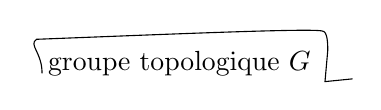
\begin{tikzpicture}[baseline=(phrase.base)]
\node[inner sep=0pt,anchor=base west] (phrase) at (0,0) {groupe topologique $G$};
\draw[line width=0.4pt]
 ([xshift=-2pt,yshift=1pt]phrase.south west)
 .. controls ([xshift=-2pt,yshift=4pt]phrase.west)
          and ([xshift=-7pt,yshift=2pt]phrase.north west)
 .. ([xshift=-4pt,yshift=4pt]phrase.north west)
 .. controls ([yshift=6pt]phrase.north)
          and ([yshift=8pt]phrase.north east)
 .. ([xshift=4pt,yshift=7pt]phrase.north east)
 .. controls ([xshift=6pt,yshift=7pt]phrase.north east)
          and ([xshift=6pt,yshift=2pt]phrase.north east)
 .. ([xshift=6pt]phrase.north east)
 -- ([xshift=5pt,yshift=-2pt]phrase.south east)
 -- ([xshift=15pt,yshift=-1pt]phrase.south east);
\end{tikzpicture}}
tel que \deleted{\unsure{$\widetilde A_0^\circ$}}\inserted{$G^\circ$} soit simplement connexe; \deleted{soit}
\deleted{\unsure{posons} $\mu=\mathrm{Centre}(\unsure{\widetilde A_0^\circ})$}
\[
(67)\qquad\Pi_1(G^\circ)=0
\]
soit
\[
(68)\qquad \mu=\mathrm{Centre}(G^\circ),\qquad\Gamma=G/G^\circ
\]
\margin{on suppose $\mu$ discret (donc $G^\circ$ s'identifie au groupe rev. universel de $G^\circ/\mu=\mathcal H^\circ$ (si $\mathcal H=G/\mu$))}
alors l'extension de groupes topologiques $G$
de $\Gamma$ par $G^\circ$ définit
\[
(69)\qquad\Gamma\longrightarrow\mathrm{Aut\,ext}(G^\circ)
\qquad(\longrightarrow\mathrm{Aut}(\mu).)
\]
et l'ens des classes d'extensions correspondantes
à une opération \inserted{extérieure} donnée de $\Gamma$ sur $G^\circ$
est de façon naturelle un torseur sous
$H^2(\Gamma,\mu)$ (s'il n'est vide, ce \unsure{qui est|qu'on a} exclu
par hypothèse de départ, en partant de $G$\ldots)
\margin{236}

\scanpage{238}
Cette catégorie d'extensions est d'ailleurs équivalente
\deleted{Elle \unsure{correspond}}
à celle des scindages d'une certaine
Gr.-catégorie définie par Sinh \inserted{via $(69)$}, dont les $\Pi_0$ et
$\Pi_1$ sont respectivement $\deleted{\unsure{\Pi_0}}\Gamma$ et $\mu$ --- laquelle
est \inserted{donc} ici scindée par la donnée de l'extension
$G$. (Dans le cas qui nous intéresse,
$\Gamma\simeq\mu\simeq\{\pm1\}$, et
cette extension est $\overline{\mathrm m}$ scindée, et correspond
à une opération d'ordre $2$ de $\Gamma$ sur $G^\circ$,
dont je doute fort que ce soit un autom intérieur.
En fait, j'ai l'impression que dans les
deux cas qui nous occupent ($\widetilde{\mathrm{GP}}(1,\mathbb C)$ et
$\widetilde A_0$) que $(69)$ est un \uline{iso}
$\Gamma=\{\pm1\}\xrightarrow{\sim}\mathrm{Autext}(G^\circ$

Ceci posé, la donnée d'un torseur sous
$\mathcal H=G/\mu$ définit $1^\circ$) un torseur sous $\Gamma$,
$\mathcal H\longrightarrow\Gamma\simeq\mathcal H/\mathcal H^\circ$; $2^\circ$) le groupoïde des
relèvements des relèvements de ce torseur
en un torseur sous $G$, qui est un
$\mu$-groupoïde \inserted{connexe} (sur lequel $\mu$ opère).
\margin{On suppose que $\Gamma$ opère \uline{trivialement} sur $\mu$ i.e. $\mu\subset\mathrm{Centre}(G)$}

Si on \deleted{\unsure{exp}} reprend en termes de fibrés
sur un espace de base $S$ on trouve
\margin{237}

\scanpage{239}
\mspage{120}
encore sur $S$ (pour tt $\mathcal H_S$-torseur topologique)
un couple $(\omega,\unsure{\mathcal R|R})$ d'un $\Gamma$-torseur, et d'
une $\mu$-gerbe sur $S$, qui sont décrits (à \unsure{isom.}
\inserted{\illegible{1} \unsure{équival.}}
\unsure{à équiv.|et équiv.} près) par $H^1(S,\Gamma)$ et $H^2(S,\mu)$
respectivement. On voudrait dégager des
conditions \inserted{sur $G$ et sur $S$} pour que l'application
\[
(70)\qquad H^1(S,\mathcal H)\longrightarrow H^1(S,\Gamma)\times H^2(S,\mu)
\]
soit bijective.
\margin{\uline{NB} $\omega$ ne dépend pas du choix de l'extension \unsure{$\widetilde G$} de $\mathcal H$ par \unsure{$\mathfrak z$|$\zeta$}${}\simeq\Pi_1(\mathcal H^\circ)$; \unsure{par contre} $\mathcal R$ en dépend (et il \unsure{faudrait} voir comment)}

Injectivité : Si l'image \inserted{d'un $\zeta\in H^1(S,\mathcal H)$,}
dans $H^2(S,\mu)$ est nulle,
l'élément de $H^1(S,\mathcal H)$ se relève en un élément $\widetilde\zeta$
de $H^1(S,\widetilde{\mathcal H}=G)$; \unsure{dont} l'image dans $H^1(S,\Gamma)$
\unsure{par} $G\longrightarrow\Gamma$ est la $\overline{\mathrm m}$ que celle de $\zeta$, donc si
elle est triviale, on voit que $\widetilde\zeta$ provient d'
un $\widetilde\zeta_0\in H^1(S,G^\circ)$. Si on sait que
$H^1(S,G^\circ)=(1)$, on gagne. Par les
marteaux-pilons d'homotopie, ça marche
si $\exists n\in\mathbb N$ avec
\[
\Pi_i(G^\circ)=0\quad\text{si}\quad i\leq n
\]
\inserted{(donc $\Pi_i(B_{G^\circ})=0$ si $i\leq n+1$)}
\deleted{$\Pi_i(S)=0$ si $i>n+1$}
\deleted{$\dim S\leq n+1$}
$S$ un CW-complexe de dim $\leq n+1$
\margin{dans le cas qui nous occupe, on peut prendre $n=2$}

Pour la surjectivité, notons que \unsure{pour|d'abord} un
\margin{238}

\scanpage{240}
élément de $H^2(S,\mu)$, l'obstruction à ce qu'il
se relève en un élément \inserted{$\zeta$} de $H^1(S,\mathcal H)$ est
dans $H^2(S,G)$ [par la suite exacte
de \unsure{coh.} associée : $1\longrightarrow\mu_S\longrightarrow G_S\longrightarrow\mathcal H_S\longrightarrow1$]
il faut exprimer qu'une certaine \deleted{\illegible{1}} gerbe
liée par $G_S$ est neutre --- brr!. Mais
partons plutôt de l'élément \inserted{\unsure{$\omega$|$\widetilde\zeta$}} de $H^1(S,\Gamma)$,
si l'extension de $\Gamma$ par \deleted{\unsure{$G^\circ$}}$\mathcal H^\circ$ est scindée, alors
on peut trouver un $\zeta_0\in H^1(S,\mathcal H_S)$ qui
donne naissance à \unsure{$\omega$}. Elle a une certaine
obstruction $\rho_0$ dans $H^2(S,\mu)$, et il s'agit
de corriger $\zeta_0$ en $\zeta$, \inserted{de} telle façon que
l'obstruction devienne $\rho\in H^2(S,\mu)$ donné.
\deleted{On dispose de} \inserted{Utilisant $\zeta_0$} pour tordre $\mathcal H_S$ en
$\mathcal H'_S$, et (via l'opération de $\mathcal H_S$ \inserted{$=G_S/\mu_S$} sur $G_S$,
compte tenu que $\mu_S\subset\mathrm{centre}\,G_S$) pour
tordre $G_S$ aussi \inserted{en $G'_S$}, d'où
\[
1\longrightarrow\mu\longrightarrow G'_S\longrightarrow\mathcal H'_S\longrightarrow1
\]
on trouve que les $\zeta$ ayant $\overline{\mathrm m}$ image dans $H^1(S,\Gamma)$
\margin{239}
